\documentclass[11pt,a4paper]{article} % Сурс - семинары по алгебре Медведя Никиты Юрьевича
\usepackage[utf8]{inputenc}
\usepackage[T2A]{fontenc}

\usepackage[english,russian]{babel}
\usepackage{amsfonts,amssymb}
\usepackage{graphicx}
\graphicspath{ {.} }

\usepackage{amsmath}
\usepackage{amsthm}
\usepackage{relsize}

\usepackage{systeme}

\usepackage{indentfirst} % Красная строка
\usepackage{fancyhdr}
\usepackage{wrapfig}
\usepackage{textcomp}

\usepackage{xcolor}% http://ctan.org/pkg/xcolor
%\usepackage{colortbl}% http://ctan.org/pkg/colortbl
\usepackage{multirow}% http://ctan.org/pkg/multirow
\usepackage{graphicx}% http://ctan.org/pkg/graphicx

\usepackage[unicode]{hyperref}

\usepackage{scontents}

% Blank formula checking
\usepackage{ifthen}
\newlength{\pheight}

\usepackage{centernot}
\usepackage{tabularx}
\usepackage{adjustbox, array, hhline}
\usepackage{makecell}

\addtolength{\textwidth}{122pt}
\addtolength{\hoffset}{-3cm}
\addtolength{\voffset}{-3cm}
\addtolength{\textheight}{170pt}

\tolerance=3000
% \flushbottom

\parindent=1cm
\def \flr#1{\left\lfloor #1 \right\rfloor}

\begin{document}
\hspace{-1.5cm} 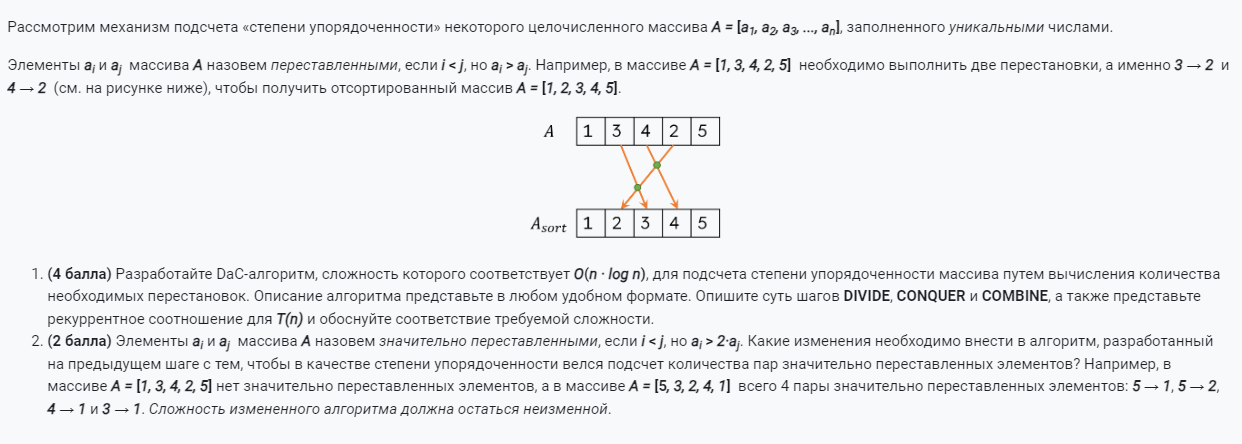
\includegraphics[scale=0.60]{a4_df.png}
\section*{Пункт 1}

\begin{tabular}{l}
    Назовём $ \textit{беспорядком} $ пару элементов массива $ a_i $ и $ a_j $, таких что $ i < j $ и $ a_i > a_j $, \\
    т.е. $ \textit{беспорядок} $ - это пара $ \textit{переставленных} $ элементов массива. \\
    Опишем алгоритм нахождения количества $ \textit{беспорядков} $ во входном массиве A на \\
    интервале $ [l; r] $ (то есть на подмассиве $ A[l; r] $): \\
    $ \textbf{DIVIDE} $ Рекурсивно найдём количество $ \textit{беспорядков} $ на интервалах $ [l; m] $ и $ [m + 1; r] $, где $ m = \flr{\frac{l + r}{2}} $. \\
    $ \textbf{CONQUER} $ Тогда для получения ответа осталось найти количество $ \textit{беспорядков} $, таких, \\
    что первый элемент пары имеет индекс от $ l $ до $ m $ включительно, а второй элемент пары имеет \\
    индекс от $ m + 1 $ до $ r $ включительно. Это верно, так как количество всех остальных возможных \\
    $ \textit{беспорядоков} $, оба индекса элементов которых принадлежат либо $ [l; m] $, либо $ [m + 1; r] $, \\
    было найдено рекурсивно. \\
    $ \textbf{COMBINE} $ Тогда ответом будет сумма количества найденных $ \textit{беспорядков} $ и количеств \\
    $ \textit{беспорядков} $, найденных рекурсивно. \\
    \\
    В условии задачи не запрещено использовать дополнительную память. \\
    Приведём пример алгоритма, решаеющего поставленную задачу и использующего \\
    $ \mathcal{O}(n) $ дополнительной памяти. \\
    Модифицируем сортировку слиянием (Merge sort) так, чтобы при слиянии \\
    подмассивов $ [l; m] $ и $ [m + 1; r] $ подсчитывалось количество $ \textit{беспорядков} $ из шага \\
    $ \textbf{CONQUER} $, а функция сортировки подмассива $ A[l; r] $ возвращала количество \\
    $ \textit{беспорядков} $ на интервале $ [l; r] $. \\
    Т.к. разрабатываемый DaC-алгоритм не должен изменять входной массив, то для работы \\
    функции сортировки потребуется создать копию массива, т.е. будет использовано \\
    $ \mathcal{O}(n) $ дополнительной памяти. В таком случае, для удобства (и понятности написанного кода) \\
    будем использовать "неэффективную" реализацию сортировки слиянием, требующую \\
    $ \mathcal{O}(n) $ дополнительной памяти. В таком случае, расход дополнительной памяти останется \\
    равным $ \mathcal{O}(n) $. \\
    \\
    Пусть на каком-то шаге сортировки необходимо слить (merge) подмассивы $ A[l; m] $ и \\
    $ A[m + 1; r] $, индексом $ l_1 $ обозначим передвигаемый индекс в подмассиве $ A[l; m] $, \\
    а индексом $ l_2 $ обозначим передвигаемый индекс в подмассиве $ A[m + 1; r] $. \\
    Если в какой-то момент $ A[l_1] > A[l_2] $, то и любой элемент в подмассиве $ A[l_1 + 1; m] $ больше \\
    элемента $ A[l_2]. $ В таком случае ответ нужно увеличить на $ m - l_1 + 1 $. При этом мы учтём все \\
    возможные $ \textit{беспорядоки} $, т.к. индекс $ l_2 $ пройдёт по всем элементам правого подмассива, \\
    а левый индекс $ l_1 $ будет двигаться вправо, пока $ A[l_1] \le A[l_2] $.
\end{tabular}

\pagebreak

Пример реализации алгоритма на языке программирования C++

(функция {\large size\_t countPermutations(const std::vector<int64\_t>\&)} )

Описанное выше обновление ответа происходит на строке с номером 36

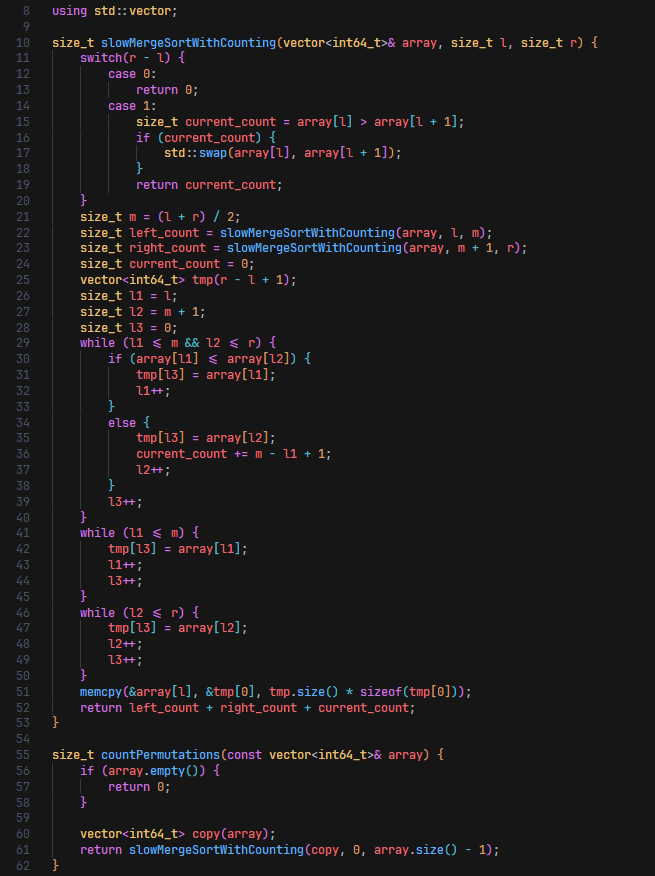
\includegraphics[scale=0.9]{a4_code_1.png}

\begin{tabular}{l}
    \\
    \\
    Функция временной сложности $ T_1(n) $ алгоритма slowMergeSortWithCounting описывается \\
    рекуррентным соотношением $ T_1(n) = 2 \cdot T_1(\frac{n}{2}) + \Theta(n) \implies $ по master-теореме \\
    $ T_1(n) = \Theta(n \log n) $ \\
    Функция временной сложности $ T(n) $ искомого алгоритма countPermutations равна \\
    $ T(n) = T_1(n) + \Theta(n) \implies T(n) = \Theta(n \log n) $.
\end{tabular}

\pagebreak

\section*{Пункт 2}

\begin{tabular}{l}
    Модифицируем функцию slowMergeSortWithCounting так, чтобы количество \\
    беспорядков шага $ \textbf{CONQUER} $ $ current\_count $ увеличивлось только для \\
    элементов $ a_i $ и $ a_j $, таких что $ a_i > 2 * a_j $. \\
    Для этого вынесем подсчёт $ current\_count $ в отдельный цикл, в котором \\
    также будет два индекса: $ l_1 $ для левого подмассива и $ l_2 $ для правого подмассива. \\
    В цикле по $ l_2 $ от $ m + 1 $ до $ r $ индекс $ l_1 $ будет увеличиваться во внутреннем цикле, \\
    пока $ l_1 \le m \wedge A[l_1] \le 2 * A[l_2] $. После остановки внутреннего цикла обновляется \\
    $ current\_count $ на величину $ m - l_1 + 1 $. Случай, когда цикл завершился из-за $ l_1 > m $ \\
    будет обработан автоматически, т.к. в таком случае $ l_1 = m + 1 \implies m - l_1 + 1 = 0 $ \\
    Таким образом на каждой итерации добавляется дополнительная работа $ \Theta(n) $ \\
    (т.к. каждый из индексов $ l_1 $ и $ l_2 $ пройдут значения от $ l $ до $ m $ и от $ m + 1 $ до $ r $) $ \implies $ \\
    У модифицированного алгоритма $ T_2(n) = 2 \cdot T_2(\frac{n}{2}) + \Theta(n) + \Theta(n) = 2 \cdot T_2(\frac{n}{2}) + \Theta(n) \implies $ \\
    $ \implies T_2(n) = \Theta(n \log n) $
    \\
    \\
\end{tabular}{l}


Пример реализации алгоритма на языке программирования C++ (на следующей странице)

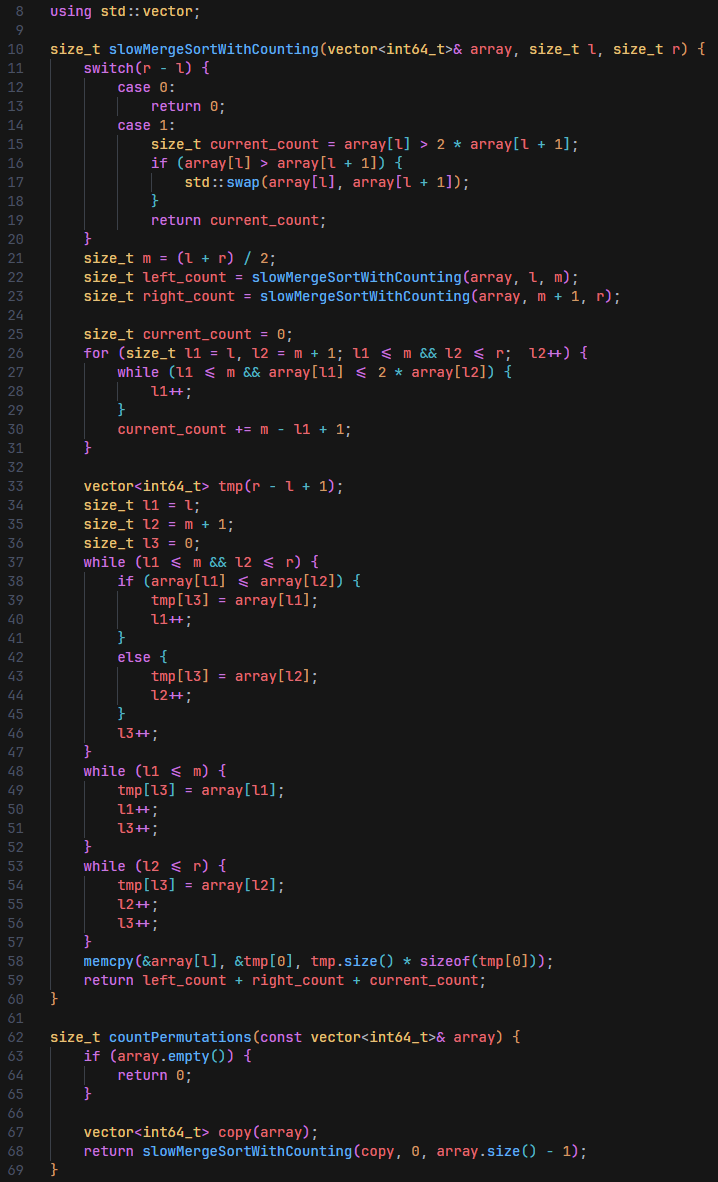
\includegraphics[scale=0.9]{a4_code_2.png}

\end{document}
